% Options for packages loaded elsewhere
\PassOptionsToPackage{unicode}{hyperref}
\PassOptionsToPackage{hyphens}{url}
\PassOptionsToPackage{dvipsnames,svgnames,x11names}{xcolor}
%
\documentclass[
  letterpaper,
  DIV=11,
  numbers=noendperiod]{scrartcl}

\usepackage{amsmath,amssymb}
\usepackage{setspace}
\usepackage{iftex}
\ifPDFTeX
  \usepackage[T1]{fontenc}
  \usepackage[utf8]{inputenc}
  \usepackage{textcomp} % provide euro and other symbols
\else % if luatex or xetex
  \usepackage{unicode-math}
  \defaultfontfeatures{Scale=MatchLowercase}
  \defaultfontfeatures[\rmfamily]{Ligatures=TeX,Scale=1}
\fi
\usepackage{lmodern}
\ifPDFTeX\else  
    % xetex/luatex font selection
    \setmainfont[]{TeX Gyre Termes}
\fi
% Use upquote if available, for straight quotes in verbatim environments
\IfFileExists{upquote.sty}{\usepackage{upquote}}{}
\IfFileExists{microtype.sty}{% use microtype if available
  \usepackage[]{microtype}
  \UseMicrotypeSet[protrusion]{basicmath} % disable protrusion for tt fonts
}{}
\makeatletter
\@ifundefined{KOMAClassName}{% if non-KOMA class
  \IfFileExists{parskip.sty}{%
    \usepackage{parskip}
  }{% else
    \setlength{\parindent}{0pt}
    \setlength{\parskip}{6pt plus 2pt minus 1pt}}
}{% if KOMA class
  \KOMAoptions{parskip=half}}
\makeatother
\usepackage{xcolor}
\usepackage[left=2.54cm,right=2.54cm,top=2.54cm,bottom=2.54cm]{geometry}
\setlength{\emergencystretch}{3em} % prevent overfull lines
\setcounter{secnumdepth}{-\maxdimen} % remove section numbering
% Make \paragraph and \subparagraph free-standing
\makeatletter
\ifx\paragraph\undefined\else
  \let\oldparagraph\paragraph
  \renewcommand{\paragraph}{
    \@ifstar
      \xxxParagraphStar
      \xxxParagraphNoStar
  }
  \newcommand{\xxxParagraphStar}[1]{\oldparagraph*{#1}\mbox{}}
  \newcommand{\xxxParagraphNoStar}[1]{\oldparagraph{#1}\mbox{}}
\fi
\ifx\subparagraph\undefined\else
  \let\oldsubparagraph\subparagraph
  \renewcommand{\subparagraph}{
    \@ifstar
      \xxxSubParagraphStar
      \xxxSubParagraphNoStar
  }
  \newcommand{\xxxSubParagraphStar}[1]{\oldsubparagraph*{#1}\mbox{}}
  \newcommand{\xxxSubParagraphNoStar}[1]{\oldsubparagraph{#1}\mbox{}}
\fi
\makeatother


\providecommand{\tightlist}{%
  \setlength{\itemsep}{0pt}\setlength{\parskip}{0pt}}\usepackage{longtable,booktabs,array}
\usepackage{calc} % for calculating minipage widths
% Correct order of tables after \paragraph or \subparagraph
\usepackage{etoolbox}
\makeatletter
\patchcmd\longtable{\par}{\if@noskipsec\mbox{}\fi\par}{}{}
\makeatother
% Allow footnotes in longtable head/foot
\IfFileExists{footnotehyper.sty}{\usepackage{footnotehyper}}{\usepackage{footnote}}
\makesavenoteenv{longtable}
\usepackage{graphicx}
\makeatletter
\newsavebox\pandoc@box
\newcommand*\pandocbounded[1]{% scales image to fit in text height/width
  \sbox\pandoc@box{#1}%
  \Gscale@div\@tempa{\textheight}{\dimexpr\ht\pandoc@box+\dp\pandoc@box\relax}%
  \Gscale@div\@tempb{\linewidth}{\wd\pandoc@box}%
  \ifdim\@tempb\p@<\@tempa\p@\let\@tempa\@tempb\fi% select the smaller of both
  \ifdim\@tempa\p@<\p@\scalebox{\@tempa}{\usebox\pandoc@box}%
  \else\usebox{\pandoc@box}%
  \fi%
}
% Set default figure placement to htbp
\def\fps@figure{htbp}
\makeatother
% definitions for citeproc citations
\NewDocumentCommand\citeproctext{}{}
\NewDocumentCommand\citeproc{mm}{%
  \begingroup\def\citeproctext{#2}\cite{#1}\endgroup}
\makeatletter
 % allow citations to break across lines
 \let\@cite@ofmt\@firstofone
 % avoid brackets around text for \cite:
 \def\@biblabel#1{}
 \def\@cite#1#2{{#1\if@tempswa , #2\fi}}
\makeatother
\newlength{\cslhangindent}
\setlength{\cslhangindent}{1.5em}
\newlength{\csllabelwidth}
\setlength{\csllabelwidth}{3em}
\newenvironment{CSLReferences}[2] % #1 hanging-indent, #2 entry-spacing
 {\begin{list}{}{%
  \setlength{\itemindent}{0pt}
  \setlength{\leftmargin}{0pt}
  \setlength{\parsep}{0pt}
  % turn on hanging indent if param 1 is 1
  \ifodd #1
   \setlength{\leftmargin}{\cslhangindent}
   \setlength{\itemindent}{-1\cslhangindent}
  \fi
  % set entry spacing
  \setlength{\itemsep}{#2\baselineskip}}}
 {\end{list}}
\usepackage{calc}
\newcommand{\CSLBlock}[1]{\hfill\break\parbox[t]{\linewidth}{\strut\ignorespaces#1\strut}}
\newcommand{\CSLLeftMargin}[1]{\parbox[t]{\csllabelwidth}{\strut#1\strut}}
\newcommand{\CSLRightInline}[1]{\parbox[t]{\linewidth - \csllabelwidth}{\strut#1\strut}}
\newcommand{\CSLIndent}[1]{\hspace{\cslhangindent}#1}

\usepackage{booktabs}
\usepackage{longtable}
\usepackage{array}
\usepackage{multirow}
\usepackage{wrapfig}
\usepackage{float}
\usepackage{colortbl}
\usepackage{pdflscape}
\usepackage{tabu}
\usepackage{threeparttable}
\usepackage{threeparttablex}
\usepackage[normalem]{ulem}
\usepackage{makecell}
\usepackage{xcolor}
\KOMAoption{captions}{tableheading}
\makeatletter
\@ifpackageloaded{caption}{}{\usepackage{caption}}
\AtBeginDocument{%
\ifdefined\contentsname
  \renewcommand*\contentsname{Tabla de contenidos}
\else
  \newcommand\contentsname{Tabla de contenidos}
\fi
\ifdefined\listfigurename
  \renewcommand*\listfigurename{Listado de Figuras}
\else
  \newcommand\listfigurename{Listado de Figuras}
\fi
\ifdefined\listtablename
  \renewcommand*\listtablename{Listado de Tablas}
\else
  \newcommand\listtablename{Listado de Tablas}
\fi
\ifdefined\figurename
  \renewcommand*\figurename{Figura}
\else
  \newcommand\figurename{Figura}
\fi
\ifdefined\tablename
  \renewcommand*\tablename{Tabla}
\else
  \newcommand\tablename{Tabla}
\fi
}
\@ifpackageloaded{float}{}{\usepackage{float}}
\floatstyle{ruled}
\@ifundefined{c@chapter}{\newfloat{codelisting}{h}{lop}}{\newfloat{codelisting}{h}{lop}[chapter]}
\floatname{codelisting}{Listado}
\newcommand*\listoflistings{\listof{codelisting}{Listado de Listados}}
\makeatother
\makeatletter
\makeatother
\makeatletter
\@ifpackageloaded{caption}{}{\usepackage{caption}}
\@ifpackageloaded{subcaption}{}{\usepackage{subcaption}}
\makeatother

\ifLuaTeX
\usepackage[bidi=basic]{babel}
\else
\usepackage[bidi=default]{babel}
\fi
\babelprovide[main,import]{spanish}
\ifPDFTeX
\else
\babelfont{rm}[]{TeX Gyre Termes}
\fi
% get rid of language-specific shorthands (see #6817):
\let\LanguageShortHands\languageshorthands
\def\languageshorthands#1{}
\usepackage{bookmark}

\IfFileExists{xurl.sty}{\usepackage{xurl}}{} % add URL line breaks if available
\urlstyle{same} % disable monospaced font for URLs
\hypersetup{
  pdftitle={Perfiles de Individualismo en la sociedad chilena},
  pdfauthor={Gabriel Cortés Paredes},
  pdflang={es},
  pdfkeywords={Individualismo, Individuación, Análisis de clases
latentes},
  colorlinks=true,
  linkcolor={blue},
  filecolor={Maroon},
  citecolor={Blue},
  urlcolor={Blue},
  pdfcreator={LaTeX via pandoc}}


\title{Perfiles de Individualismo en la sociedad chilena}
\author{Gabriel Cortés Paredes}
\date{}

\begin{document}
\maketitle
\begin{abstract}
Este artículo busca identificar, a partir de un modelo de clases
latentes, los perfiles de individualismo presentes en la sociedad
chilena. Se entiende aquí individualismo como el conjunto de
concepciones que tratan a la persona como el responsable principal de su
propia vida, definiendo el lugar del individuo en la sociedad. Esta
conceptuzalización permite comprender el individualismo como un producto
de procesos socihistóricos de individuación, que varían no solo entre
culturas sino también dentro de una misma sociedad.

Utilizando datos secundarios de la 7ma Ola de la Encuesta Mundial de
Valores en Chile (2018), se llevó a cabo un Análisis de Clases Latentes.
Este análisis reveló cuatro perfiles distintos de individualismo:
Autoritario, Conservador, Liberal y Estratégico. Aunque los cuatro
perfiles muestran similutdes en sus niveles de independneica e
interdependencia, difieren fundamentalmente en las esferas donde la
individualidad se considera legítima.

Los resultados de esta investigación permiten, por un lado,
problematizar la posibilidad de ubicar a la sociedad chilena en un
continuo entre individualismo y colectivismo. Por otro, matiza las
interpretaciones unívocas sobre la existencia de una forma única de
individualismo en Chile.
\end{abstract}


\setstretch{1.15}
\section{Introducción}\label{introducciuxf3n}

Desde los inicios de las ciencias sociales, la pregunta por cómo las
sociedades se mantienen unidas ha sido central para la reflexión
sociológica. Aunque la modernidad se asoció con una mayor autonomía
individual, el individualismo fue visto con sospecha por figuras
fundacionales. Si bien este nuevo fenómeno estuvo lejos de significar el
fin de la sociedad, autores como Alexis de Tocqueville y Émile Durkheim
advirtieron que un individualismo extremo puede derivar en patologías
sociales, como la fragmentación de los vínculos comunitarios.

Esta preocupación adquiere especial relevancia en el contexto
contemporáneo, marcado por una acumulación de crisis sociales, políticas
y económicas que tensionan la cohesión social a escala global. En Chile,
la cuestión se vuelve particularmente visible tras el ciclo abierto por
la crisis social de 2019, las frustradas experiencias constituyentes y
crisis sucesivas ---sanitaria, migratoria y de seguridad---, que han
reactivado el debate sobre la calidad de los lazos cívicos, sociales y
comunitarios en el país (\citeproc{ref-mideso_informe_2020}{Ministerio
de Desarrollo Social y Familia 2020};
\citeproc{ref-castillo_cohesion_2022}{Castillo, Espinoza, y Barozet
2022}; \citeproc{ref-salazar-xirinachs_repensar_2023}{Salazar-Xirinachs
2023}).

Chile se ha caracterizado por el avance de reformas neoliberales
profundas durante la dictadura militar (1973--1990) y su posterior
consolidación en democracia. Dichas transformaciones excedieron el plano
económico e instalaron un discurso hegemónico que enfatiza el esfuerzo
personal, la competencia y la meritocracia como vías legítimas de logro.
Políticas públicas en educación, salud y bienestar reforzaron la
responsabilidad individual, favoreciendo subjetividades centradas en la
agencia personal (\citeproc{ref-araujo2012}{Araujo y Martuccelli 2012}),
legitimando desigualdades económicas
(\citeproc{ref-castillo_socialization_2024}{Castillo et~al. 2024}),
favoreciendo el actuar estratégico (\citeproc{ref-araujo2014}{Araujo y
Martuccelli 2014}) y, eventualmente, inhibiendo el cambio político
(\citeproc{ref-pnud2024}{PNUD 2024}).

Desde esta perspectiva, la presencia de un~\emph{individualismo asocial}
(\citeproc{ref-pnud2024}{PNUD 2024}) operaría como fuerza disgregadora
de lazos sociales y ciudadanos, configurándose como un desafío para la
mantención de la cohesión social en Chile. En este contexto, este
artículo busca aportar a la discusión empírica identificando los
distintos~\textbf{perfiles de individualismo}~presentes en la sociedad
chilena.

El estudio del individualismo ha estado dominado por la psicología
cultural, especialmente a partir del enfoque popularizado por Geert
Hofstede en los años ochenta. En su formulación, el individualismo y el
colectivismo constituyen polos de un continuo unidimensional que
permitiría distinguir entre culturas individualistas y colectivistas
(\citeproc{ref-oyserman2002}{Oyserman, Coon, y Kemmelmeier 2002};
\citeproc{ref-yoon2010}{Yoon 2010}). Las primeras se caracterizan por
lazos poco estrechos y expectativas de autosuficiencia individual y
familiar; las segundas, por la integración temprana en grupos
cohesionados que brindan protección a cambio de lealtad
(\citeproc{ref-yoon2010}{Yoon 2010}).

El fenómeno del individualismo ha sido abordado principalmente desde la
psicología cultural, particularmente desde el enfoque popularizado por
Geert Hofstede en la década de 1980. Para Hofstede, el individualismo es
el polo de un espectro continuo y unidimensional que tiene en su otro
extremo al colectivismo. De tal modo, sería posible distinguir entre
culturas individualistas y culturas colectivistas
(\citeproc{ref-oyserman2002}{Oyserman, Coon, y Kemmelmeier 2002};
\citeproc{ref-yoon2010}{Yoon 2010}). Las sociedades individualistas se
caracterizarían por la existencia de lazos poco estrechos entre sus
individuos, de quienes se espera se hagan cargos de sí mismos y de su
familia inmediata. Las sociedades colectivistas, en tanto, se definen
porque sus miembros están integrados desde su nacimiento a grupos
fuertemente cohesionados que los protegen a lo largo de sus vidas a
cambio de una lealtad incuestionable (\citeproc{ref-yoon2010}{Yoon
2010}).

Pese a su influencia, este enfoque ha recibido críticas por su vaguedad
conceptual ---a veces tratado como un ``catch-all'' para explicar toda
diferencia cultural (\citeproc{ref-voronov2002}{Voronov y Singer
2002})--- y por su sesgo normativo, que asocia el individualismo con la
modernidad y el desarrollo (\citeproc{ref-martuccelli2010}{Martuccelli
2010}; \citeproc{ref-voronov2002}{Voronov y Singer 2002};
\citeproc{ref-wang2010}{Wang y Liu 2010}). También se le objeta la
imprecisión en la definición de ``colectivos'' ---sin distinguir con
claridad entre grupos, colectivos y comunidades
(\citeproc{ref-brewer2007}{Brewer y Chen 2007};
\citeproc{ref-moemeka1998}{Moemeka 1998};
\citeproc{ref-oyserman2002}{Oyserman, Coon, y Kemmelmeier 2002})--- y la
frecuente confusión entre niveles de análisis (cultural vs.~individual),
a menudo solapando cofundiéndose a nivel operacional y teórico con
conceptos como el \emph{self-construal} (\citeproc{ref-cross2011}{Cross,
Hardin, y Gercek-Swing 2011}; \citeproc{ref-voronov2002}{Voronov y
Singer 2002}).

A ello se suman problemas de operacionalización
(\citeproc{ref-brewer2007}{Brewer y Chen 2007};
\citeproc{ref-oyserman2002}{Oyserman, Coon, y Kemmelmeier 2002}). Brewer
y Chen (\citeproc{ref-brewer2007}{2007}) señalan la existencia de una
asimetría habitual en las operacionalizaciones de los conceptos:
mientras el individualismo se mide con ítems sobre identidad y agencia
personal, el colectivismo suele capturarse como un sistema de valores.

Estas discrepancias conceptuales podrían explicar las anomalías
observados en varios de estos estudios, como que los individualistas
pueden ser tanto o más colectivistas que colectivistas mismos
(\citeproc{ref-oyserman2002}{Oyserman, Coon, y Kemmelmeier 2002}), o que
en determinados contextos los colectivistas actúan de manera
individualista (\citeproc{ref-voronov2002}{Voronov y Singer 2002}).

En el plano agregado, Chile ilustra esas tensiones. Bajo la definición
de Hofstede, la sociedad chilena ha sido clasificada como colectivista
(\citeproc{ref-leonquillas2022}{León Quillas, Rueda Rodríguez, y
Hernández Rodríguez 2022}; \citeproc{ref-rojas2008}{Rojas-Méndez et~al.
2008}). Esto concuerda con hallazgos que reportan altos niveles de
colectivismo, sea como opuesto al individualismo
(\citeproc{ref-oyserman2002}{Oyserman, Coon, y Kemmelmeier 2002}) o como
self-construal interdependiente (\citeproc{ref-benavides2020}{Benavides
y Hur 2020}). Sin embargo, otras mediciones muestran niveles de
individualismo en Chile que son comparables o superiores a los de
sociedades típicamente individualistas, como Estados Unidos
(\citeproc{ref-oyserman2002}{Oyserman, Coon, y Kemmelmeier 2002}) o
Noruega (\citeproc{ref-kolstad2009}{Kolstad y Horpestad 2009}).

Surge así una doble pregunta: ¿es realmente una sociedad colectivista?,
y si no lo es, ¿hasta qué punto es una sociedad individualista? La
propuesta de esta investigación es que, con el fin de responder esta
pregunta, es necesario dar un giro hacia una perspectiva teórica que
provea el lenguaje para describir el individualismo chileno.
Particularmente, este artículo buscará responder esta pregunta a través
del lente de la teoría de la individualización y, particularmente, desde
la sociología del individuo.

Desde fines de los noventa, la teoría de la individualización ha sido un
marco ampliamente utilizado en las ciencias sociales para analizar
transformaciones culturales, sociales y económicas
(\citeproc{ref-yopo2013}{Yopo 2013}), aplicándose a temáticas como
género y familia (\citeproc{ref-murray2022}{Murray y Tizzoni 2022}),
religión (\citeproc{ref-baeza2022}{Baeza y Imbarack 2022};
\citeproc{ref-cortesparedes_autonomia_2022}{Cortés Paredes 2022}),
trabajo (\citeproc{ref-soto2021}{Soto, Stecher, y Frías 2021}),
seguridad (\citeproc{ref-trebilcock2019}{Trebilcock y Luneke 2019}),
discapacidad (\citeproc{ref-solsona-cisternas2023}{Solsona-Cisternas
2023}) y educación (\citeproc{ref-canalesceron2021}{Canales Cerón,
Orellana Calderón, y Guajardo Mañán 2021};
\citeproc{ref-pinheiro2023}{Pinheiro, Di Leo, y Varela 2023}). No
obstante, se ha advertido su adopción a veces acrítica, con escasa
atención a especificidades nacionales y latinoamericanas y con limitada
incorporación de variables sociodemográficas que permitan identificar
diferencias entre grupos (\citeproc{ref-gayo_individuo_2017}{Gayo 2017};
\citeproc{ref-yopo2013}{Yopo 2013}).

Sin embargo, se ha advertido que muchas de las investigaciones que
siguen esta línea teórica lo hacen a través de una aproximación acrítica
a las claves interpretativas de la teoría, sin llegar a dar cuenta de
las particularidades de estos procesos en Chile y en América Latina. Por
otro lado, se ha observado que en los estudios que utilizan esta
perspectiva teórica rara vez se usan variables sociodemográficas de
manera explicativa, descuidando posibles diferencias entre grupos
sociales (\citeproc{ref-gayo_individuo_2017}{Gayo 2017}).

Reconocer estas limitaciones es crucial, ya que existe el riesgo de
asumir una individuación homogénea dentro de la sociedad, sin
contrastación empírica suficiente, ya sea por imprecisiones conceptual
(\citeproc{ref-yopo2013}{Yopo 2013}) o por déficits metodológicos
(\citeproc{ref-gayo_individuo_2017}{Gayo 2017}).Esta brecha existe pese
al consenso aparente de que la individuación es un proceso que diverge
no solo entre culturas, sino también dentro de una misma sociedad
(\citeproc{ref-martuccelli2018}{Martuccelli 2018}).

Ante esto, el siguiente artículo busca abordar estas diferencias no solo
de manera declarativa a nivel teórico, sino identificarlas
empíricamente. A continuación, se presenta el marco conceptual y las
definiciones centrales de esta investigación; luego, al estrategia
metodológica; posteriormente, los hallazgos, caracterizando los perfiles
identificados. Finalmente, se introduce discuten los resultados a la luz
del modelo teórico y las limitaciones del estudio, junto con
proyecciones para futuras investigaciones.

\section{El Individualismo desde la Sociología del
Individuo}\label{el-individualismo-desde-la-sociologuxeda-del-individuo}

¿Es Chile una sociedad colectivista? Si no lo es, ¿qué forma adopta el
individualismo en la sociedad chilena? Abordar estas preguntas desde la
psicología cultural puede conducir ---como advierte Martuccelli--- a un
``relato de la insuficiencia'' (``Chile no es un país individualista'')
o a un relato del ni-ni (``Chile no es ni individualista ni
colectivista'') (\citeproc{ref-martuccelli2010}{Martuccelli 2010}).

Para escapar de estas trampas y ganar capacidad descriptiva, se propone
el giro hacia la sociología del individuo desarrollada por Danilo
Martuccelli (\citeproc{ref-araujo2012}{Araujo y Martuccelli 2012},
\citeproc{ref-araujo2014}{2014}, \citeproc{ref-araujo2020a}{2020b};
\citeproc{ref-martuccelli2010}{Martuccelli 2010},
\citeproc{ref-martuccelli2018}{2018}). La ventaja de adoptar esta
perspectiva es que ofrece un marco unificador que permite rescatar los
aportes de otras disciplinas a la descripción teórica y empírica del
individualismo, a la vez que ofrece un lenguaje apropiado para las
particularidades del individualismo chileno.

En esta perspectiva, la modernidad instala una representación hegemónica
de un individuo soberano en dos sentidos: (i) dueño de sí
---independiente, autónomo, singular--- y (ii) capaz de fundamentar el
orden social y la soberanía colectiva a partir de su racionalidad. Este
individuo se ubica en el centro del pacto social, en lo que Martuccelli
denomina individualismo institucional, que se compone de tres
características principales (\citeproc{ref-martuccelli2018}{Martuccelli
2018}):

\begin{enumerate}
\def\labelenumi{\roman{enumi})}
\item
  una separación tajante entre holismo e individualismo, que legitima la
  individualidad y la acción individual en todas las esferas de la vida
  social
\item
  Una concepción atomizada de la persona, prexistente a sus lazos
  sociales
\item
  la primacía de las instituciones en los procesos de individuación,
  poniendo la autonomía como valor primordial de estos procesos.
\end{enumerate}

Las lecturas se límitan a entender el individualismo como este modelo
universal suelen negar la existencia de individuos, individualización o
individualismo allí donde el patrón no calza
(\citeproc{ref-martuccelli2018}{Martuccelli 2018}). En cambio, la
sociología del individuo permite pluralizar el fenómeno y describir sus
configuraciones concretas. Sobre esa base, adoptamos la siguiente
definición que, si bien rescata la dimensiones del individualismo
institucional, se aleja de pretensiones unívocas y se abre a potenciales
variantes.

De tal modo, se entenderá como individualismo al conjunto de
concepciones que tratan a la persona como el responsable principal de su
propia vida. Como tal, el individualismo define el lugar del individuo
en la sociedad al (i) legitimar su acción en distintas esferas, (ii)
sostener representaciones de mayor o menor independencia o
interdependencia, y (iii) poniendo en relieve distintos valores
predominantes, como la autonomía o la seguridad.

A continuación, se definirán las principales dimensiones que emergen
desde esta definición.

\subsection{Legitimidad de la acción
individual}\label{legitimidad-de-la-acciuxf3n-individual}

La legitimidad de la acción individual hace referencia a las creencias
sobre la agencia de los individuos en el mundo social
(\citeproc{ref-brewer2007}{Brewer y Chen 2007}) y la legitimidad de
acciones individualizadas en las esferas de la economía, la política y
las emociones (\citeproc{ref-cortois2018}{Cortois y Laermans 2018}). Una
mayor legitimidad de la acción individual se relaciona a una mayor
valoración de la individualidad, la cual se define como el ``grado de
diferenciación o de singularización reconocido o legítimamente alcanzado
por un individuo dentro de un colectivo''
(\citeproc{ref-martuccelli2018}{Martuccelli 2018}).

El individualismo moderno ha sido institucionalizado principalmente en 3
esferas: la económica, la política y la afectiva
(\citeproc{ref-cortois2018}{Cortois y Laermans 2018};
\citeproc{ref-martuccelli2018}{Martuccelli 2018}). En la esfera
económica, el individualismo legitima la acción individual estratégica,
poniendo los medios por sobre los fines. En cambio, en la esfera
política, el individualismo se expresa como la obligación de tratar al
otro como un fin en sí mismo. Por último, en la esfera afectiva, la
acción individual se entiende como un medio para la expresión auténtica
del yo (\citeproc{ref-cortois2018}{Cortois y Laermans 2018}).

La hipótesis de esta artículo es que determinadas sociedades, o grupos
de individuos dentro de estas, pueden legitimar la acción individual en
algunas esferas, pero no necesariamente en otros. Por ejemplo, grupos
conservadores podrían aceptar la acción individual en la esfera
económica, pero no en la política o la afectiva. En cambio, grupos
liberales podrían aceptar la acción individual en todas las esferas,
pero con distintos grados de legitimidad.

\subsection{Representaciones culturales del
Individuo}\label{representaciones-culturales-del-individuo}

Son las diversas concepciones en torno a las que se pueden definir las
identidades de los individuos en relación a sus grupos de referencia
(\citeproc{ref-brewer2007}{Brewer y Chen 2007}). Al respecto, es posible
distinguir entre representaciones independientes, relacionales y
colectivas (\citeproc{ref-brewer2007}{Brewer y Chen 2007}).

La representación independiente es aquella en que el individuo se
concibe como un ente atomizado y prexistente a sus lazos sociales.
Aunque esta concepción se ha considerado como propia de las culturas
individualistas (\citeproc{ref-benavides2020}{Benavides y Hur 2020};
\citeproc{ref-cross2011}{Cross, Hardin, y Gercek-Swing 2011}), tal idea
ha sido problematizada teórica (\citeproc{ref-voronov2002}{Voronov y
Singer 2002}) y empíricamente (\citeproc{ref-benavides2020}{Benavides y
Hur 2020}; \citeproc{ref-kolstad2009}{Kolstad y Horpestad 2009}).
Además, la persistencia de los llamados valores asiáticos en esas
sociedades, que conceptualizan al individuo como inseparable de sus
lazos sociales (\citeproc{ref-zhai2022}{Zhai 2022}), y la
conceptualización de un híper-actor relacional en la sociedad chilena
(\citeproc{ref-araujo2020a}{Araujo y Martuccelli 2020b}), sugieren la
posibilidad de individualismos que difieren de las representaciones
independientes.

De tal modo, se podrían identificar, además, representaciones
relacionales y representaciones colectivas
(\citeproc{ref-brewer2007}{Brewer y Chen 2007}). En las primeras, la
identidad del individuo se define por sus relaciones cercanas, tales
como la familia o los amigos. En las segundas, en tanto, es la
pertenencia a colectivos sociales más abstractos -- esto es, grupos
nacionales, regionales, étnicos o religiosos -- lo que define a la
identidad individual (\citeproc{ref-brewer2007}{Brewer y Chen 2007}).

La hipótesis de este artículo se alinea con las investigaciones de
Kathya Aruajo y Danilo Martuccelli (\citeproc{ref-araujo2012}{2012}),
que definen con al individualismo chileno como uno predominantemente
relacional. Sin embargo, y en línea con las investigaciones sobre
\emph{self-construal} en la sociedad chilena
(\citeproc{ref-benavides2020}{Benavides y Hur 2020};
\citeproc{ref-kolstad2009}{Kolstad y Horpestad 2009}), se espera
igualmente encontrar altos niveles de representaciones independientes.

\subsection{Valores}\label{valores}

Por último, la tercera dimensión del individualismo se refiere a la
importancia relativa que se le otorga en una sociedad a diversos valores
e imperativos individuales o colectivos
(\citeproc{ref-brewer2007}{Brewer y Chen 2007}), los cuales son
producidos por procesos sociohistóricos de individuación
(\citeproc{ref-martuccelli2018}{Martuccelli 2018}). En el contexto del
individualismo institucional, el principal valor para el individuo es la
autonomía (\citeproc{ref-martuccelli2010}{Martuccelli 2010}), la que es
promovida a través de un entramado institucional
(\citeproc{ref-martuccelli2018}{Martuccelli 2018}) que promueve que los
individuos se constituyen a sí mismos, planifiquen su propia vida y
acepten la responsabilidad de si fracasan
(\citeproc{ref-robles2001}{Robles 2001}). Es, pues, una individuación
reflexiva en la que los individuos se definen por el imperativo de
ejercer control de sus destinos y tomar decisiones de manera autónoma
(\citeproc{ref-robles2001}{Robles 2001};
\citeproc{ref-silvapalacios2015}{Silva Palacios 2015}).

Sin embargo, también se han planteado visiones críticas a esta
concepción, particularmente desde América Latina
(\citeproc{ref-araujo2012}{Araujo y Martuccelli 2012};
\citeproc{ref-robles2001}{Robles 2001}). No toda individuación sería
reflexiva, ya que muchos individuos podrían experimentarla de forma
delegativa, como una imposición (\citeproc{ref-silvapalacios2015}{Silva
Palacios 2015}); no como un mundo de posibilidades, sino como uno lleno
de incertidumbres. Los individuos, de tal modo, deben enfrentar las
inseguridades ontológicas de la vida social a partir de sus propias
habilidades bajo el imperativo de ``arréglatelas como puedas''
(\citeproc{ref-araujo2014}{Araujo y Martuccelli 2014};
\citeproc{ref-robles2001}{Robles 2001}). Frente a esto, la valorización
de la autonomía se desplaza por la búsqueda de seguridad como valor
principal de esta forma de individuación
(\citeproc{ref-silvapalacios2015}{Silva Palacios 2015}).

La hipótesis de esta investigación es que en la sociedad chilena ha
predominado una individuación delegativa que enfatiza valores como la
seguridad por sobre la autonomía. No obstante, es posible que en grupos
con mayores niveles de bienestar o estatus socioeconómico predomine una
individuación reflexiva que enfatice la autonomía.

La propuesta conceptual planteada en esta sección se resume en el
Figura~\ref{fig-esquema}.

\begin{figure}[H]

\centering{

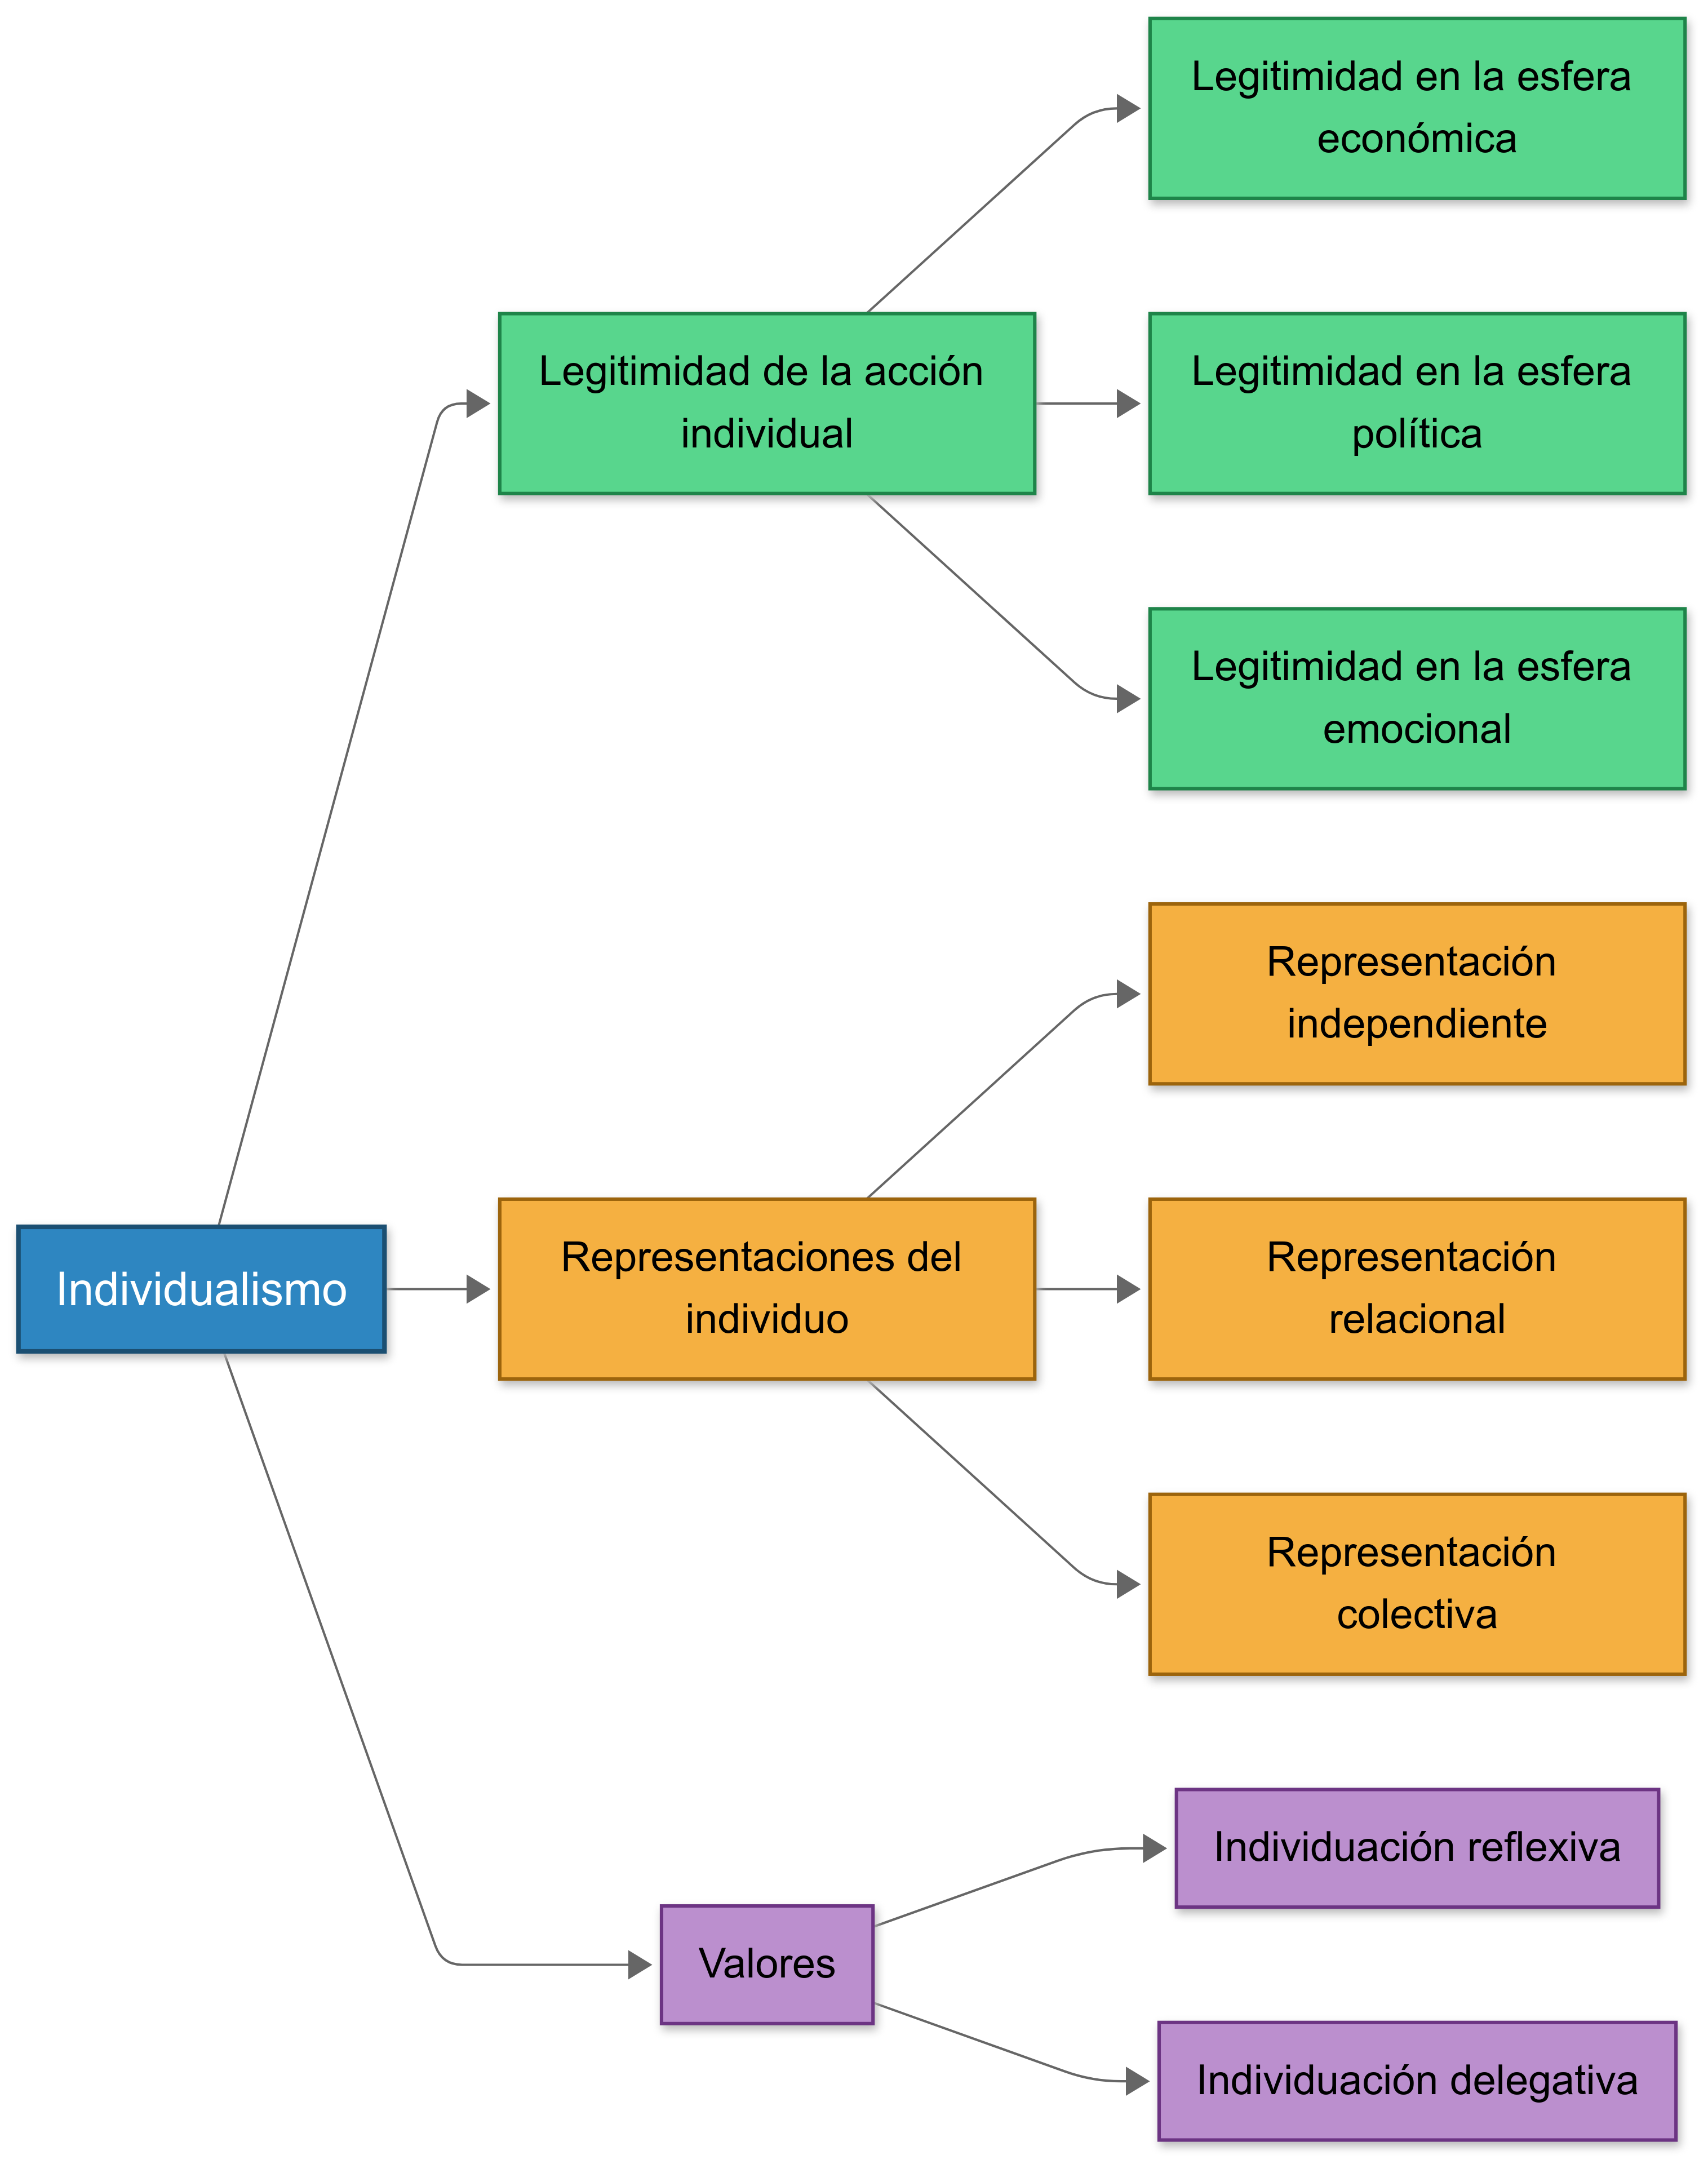
\includegraphics[width=0.6\linewidth,height=\textheight,keepaspectratio]{input/images/esquema-conceptual.png}

}

\caption{\label{fig-esquema}Esquema conceptual propuesto}

\end{figure}%

\section{Estrategia metodológica}\label{estrategia-metodoluxf3gica}

\subsection{Datos}\label{datos}

La investigación consistió en un estudio de tipo cuantitativo a partir
de datos secundarios recolectados originalmente para la séptima ola de
la Encuesta Mundial de Valores, la más reciente hasta la fecha. Este
instrumento proporciona una muestra representativa a nivel nacional, con
indicaores relevantes sobre valores y creencias sociales, políticas y
económicas de la población, posibilitando la construcción de un modelo
que identifique perfiles de individualismo.

El trabajo de campo se llevó a cabo en los meses de enero y febrero de
2018, con una muestra compuesta por 1.000 personas mayores de 18 años,
seleccionadas mediante un proceso de muestreo multietápico de tres
niveles. La muestra es representativa a nivel nacional, así como de
áreas urbanas y rurales.

\subsection{Indicadores}\label{indicadores}

Se entenderá al individualismo como una variable latente y categórica,
construida de manera inductiva a partir de un conjunto de indicadores
operacionalizados en base de las definiciones teóricas previamente
expuestas. La Tabla~\ref{tbl-indicadores} presenta un resumen de los
indicadores seleccionados.

\subsubsection{Legitimidad de la acción
individual}\label{legitimidad-de-la-acciuxf3n-individual-1}

La legitimidad de la acción individual se midió en tres esferas:

\begin{itemize}
\item
  En la \textbf{esfera económica}, se seleccionaron indicadores que
  miden la legitimidad de acciones estratégicas destinadas a obtener
  beneficios personales, incluso si estas acciones van en contra de las
  normas sociales. El énfasis aquí se centra en la legitimidad de poner
  los fines por sobre los medios. Además, se incluye un indicador que
  evalúa la valoración de la competencia.
\item
  En la \textbf{esfera política}, se incluyeron indicadores relacionados
  con la importancia atribuida a la igualdad de ingresos, la igualdad de
  género y los derechos civiles en una democracia.
\item
  En la \textbf{esfera afectiva}, se incluyeron indicadores relaciones
  con la legitimdiad de prácticas individualizadas en las esferas de la
  sexualidad y el amor, tales como la homosexualidad, el divorcio y las
  relaciones sexuales premaritales.
\end{itemize}

Estos 9 ítems corresponden a escalas del 1 al 10. Dado que el análisis
de clases latentes, como se introducirá más adelante, requiere que los
indicadores del modelo sean categóricos, se ha optado por dicotomizar
estas variables. De tal modo, los valores iguales o inferiores a 5 se
consideraron como una baja justificación de las acciones mencionadas,
mientras que los valores superiores a 5 se entendieron como una alta
justificación.

\subsubsection{Representaciones del
individuo}\label{representaciones-del-individuo}

Se midieron tres formas de representaciones culturales del individuo:

\begin{itemize}
\item
  Para medir las \textbf{representaciones independientes} se seleccionó
  un indicador sobre el grado de control percibido sobre la propia vida,
  en una escala del 1 al 10, donde 1 representa ``ningún control'' y 10
  ``una gran cantidad de control''. El ítem ha sido recodificado de modo
  que los valores iguales o inferiores a 5 representen un bajo control
  sobre la propia vida, mientras que los valores superiores a 5 se
  entienden como un alto control.
\item
  Las \textbf{representaciones relacionales} se midió a través del grado
  de acuerdo con la afirmación ``una de mis metas en la vida ha sido que
  mis padres estén orgullosos de mí''. Se trata de una escala Likert de
  4 categirías, por lo que se optó por mantener la codificación original
  y reducir la pérdida de varianza.
\item
  Las \textbf{representaciones colectivas} se midió a través del grado
  de cercanía que siente con el país. Al igual que el ítem anterior, se
  trata de una escala Likert de 4 categorías, por lo que mantuvo la
  codficación original.
\end{itemize}

\subsubsection{Valores}\label{valores-1}

El indicador seleccionado consisnte en la pregunta \emph{la mayoría de
las personas consideran que tanto la libertad como la seguridad son
importantes, pero si tuviera que elegir una, ¿cuál consideras que es más
importante?} Este indicador proporciona una forma sencilla de determinar
si la autonomía es el valor principal para los individuos o si ve
desplazada por el deseo de seguridad.

\begingroup\fontsize{10}{12}\selectfont

\begin{longtable}[t]{>{\raggedright\arraybackslash}p{3cm}>{\raggedright\arraybackslash}p{8cm}>{\raggedright\arraybackslash}p{3cm}}

\caption{\label{tbl-indicadores}Descripción indicadores}

\tabularnewline

\toprule
\multicolumn{1}{c}{Dimensión} & \multicolumn{1}{c}{Indicadores} & \multicolumn{1}{c}{Recodificación}\\
\midrule
\addlinespace[0.3em]
\multicolumn{3}{l}{\textbf{Legitimidad de la individualidad}}\\
 &  & 1. Alta acuerdo\\
\cmidrule{3-3}\nopagebreak
 & \multirow{-2}{8cm}{\raggedright\arraybackslash La competencia es buena o perjudicial} & 2. Baja acuerdo\\
\cmidrule{2-3}\nopagebreak
 &  & 1. Alta justificación\\
\cmidrule{3-3}\nopagebreak
 & \multirow{-2}{8cm}{\raggedright\arraybackslash Evitar el pago de pasaje en el transporte público} & 2. Baja justificación\\
\cmidrule{2-3}\nopagebreak
 &  & 1. Alta justificación\\
\cmidrule{3-3}\nopagebreak
\multirow{-6}{3cm}[1\dimexpr\aboverulesep+\belowrulesep+\cmidrulewidth]{\raggedright\arraybackslash Legitimidad individualismo utilitario} & \multirow{-2}{8cm}{\raggedright\arraybackslash Exigir beneficios del gobierno a los que no se tiene derecho} & 2. Baja justificación\\
\cmidrule{1-3}\pagebreak[0]
 &  & 1. Alta importancia\\
\cmidrule{3-3}\nopagebreak
 & \multirow{-2}{8cm}{\raggedright\arraybackslash El Estado hace que los ingresos de las personas sean iguales} & 2. Baja importancia\\
\cmidrule{2-3}\nopagebreak
 &  & 1. Alta importancia\\
\cmidrule{3-3}\nopagebreak
 & \multirow{-2}{8cm}{\raggedright\arraybackslash Las mujeres tienen los mismos derechos que los hombre} & 2. Baja importancia\\
\cmidrule{2-3}\nopagebreak
 &  & 1. Alta importancia\\
\cmidrule{3-3}\nopagebreak
\multirow{-6}{3cm}[1\dimexpr\aboverulesep+\belowrulesep+\cmidrulewidth]{\raggedright\arraybackslash Legitimidad individualismo moral} & \multirow{-2}{8cm}{\raggedright\arraybackslash Los derechos civiles protegen la libertad de la gente contra la opresión del Estado} & 2. Baja importancia\\
\cmidrule{1-3}\pagebreak[0]
 &  & 1. Alta justificación\\
\cmidrule{3-3}\nopagebreak
 & \multirow{-2}{8cm}{\raggedright\arraybackslash La homosexualidad} & 2. Baja justificación\\
\cmidrule{2-3}\nopagebreak
 &  & 1. Alta justificación\\
\cmidrule{3-3}\nopagebreak
 & \multirow{-2}{8cm}{\raggedright\arraybackslash El divorcio} & 2. Baja justificación\\
\cmidrule{2-3}\nopagebreak
 &  & 1. Alta justificación\\
\cmidrule{3-3}\nopagebreak
\multirow{-6}{3cm}[1\dimexpr\aboverulesep+\belowrulesep+\cmidrulewidth]{\raggedright\arraybackslash Legitimidad individualismo expresivo} & \multirow{-2}{8cm}{\raggedright\arraybackslash Tener relaciones sexuales antes del matrimonio} & 2. Baja justificación\\
\cmidrule{1-3}\pagebreak[0]
\addlinespace[0.3em]
\multicolumn{3}{l}{\textbf{Concepciones del Individuo}}\\
 &  & 1. Un gran control\\
\cmidrule{3-3}\nopagebreak
\multirow{-2}{3cm}{\raggedright\arraybackslash Representación Independiente} & \multirow{-2}{8cm}{\raggedright\arraybackslash ¿Cuánta libertad de elegir y de control siente usted que tiene sobre la forma en que le resulta su vida?} & 2. Nada de control\\
\cmidrule{1-3}\pagebreak[0]
 &  & 1. Muy de acuerdo\\
\cmidrule{3-3}\nopagebreak
 &  & 2. De acuerdo\\
\cmidrule{3-3}\nopagebreak
 &  & 3. En desacuerdo\\
\cmidrule{3-3}\nopagebreak
\multirow{-4}{3cm}{\raggedright\arraybackslash Representación Relacional} & \multirow{-4}{8cm}{\raggedright\arraybackslash Una de mis metas en la vida ha sido que mis padres estén orgullosos de mi} & 4. Muy en desacuerdo\\
\cmidrule{1-3}\pagebreak[0]
 &  & 1. Muy cercano\\
\cmidrule{3-3}\nopagebreak
 &  & 2. Cercano\\
\cmidrule{3-3}\nopagebreak
 &  & 3. Poco cercano\\
\cmidrule{3-3}\nopagebreak
\multirow{-4}{3cm}{\raggedright\arraybackslash Representación Colectiva} & \multirow{-4}{8cm}{\raggedright\arraybackslash Cercanía con Chile} & 4. Nada cercano\\
\cmidrule{1-3}\pagebreak[0]
\addlinespace[0.3em]
\multicolumn{3}{l}{\textbf{Valores e imperativos}}\\
 &  & 1. La Libertad\\
\cmidrule{3-3}\nopagebreak
\multirow{-2}{3cm}{\raggedright\arraybackslash Valor principal} & \multirow{-2}{8cm}{\raggedright\arraybackslash Considera más importante} & 2. La seguridad\\
\bottomrule

\end{longtable}

\endgroup{}

\subsection{Método}\label{muxe9todo}

Se empleó un análisis de clases latentes (LCA) para identificar los
perfiles de individualismo en la sociedad chilena. El LCA es un modeleo
de variables latentes categóricas, lo que permite identificar
diferencias cualitativas y principios de organización dentro de la
población (\citeproc{ref-collins2010}{Collins y Lanza 2010}).

En contraste a las técnicas estadísticas más utilizadas, el análisis de
clases latente se suele considerar como una \emph{aproximación orientada
a la persona} (\citeproc{ref-collins2010}{Collins y Lanza 2010}). Etsta
forma de abordar el análsisis estadístico se diferencia en que no busca
establecer relaciones entre variables, sino que tiene como objetivo
producir resultados interpretables a nivel del inviduo, brindando
información sobre los patrones generales y el comportamiento de las
personas (\citeproc{ref-bergman2015}{Bergman y Lundh 2015}). De tal
modo, el LCA ofrece la oportunidad de llevar a cabo una sociología a
nivel del individuo, posibilitando mapear los procesos estructurales de
individuación en Chile. Esto permitiría obtener una versión menos
unívoca del individualismo chileno, desarrollando una tipología que
identifique divergencias y difracciones de este fenómeno en la sociedad
chilena.

El análisis se realizó utilizando el paquete \textbf{poLCA}
(\textbf{po}lytomous Variable \emph{L}atent \emph{C}lass
\emph{A}nalysis) en R. Este paquete permite especificar modelos de
clases latentes de manera eficiente con solo unas pocas líneas de código
y proporciona información valiosa sobre el tamaño de cada clase latente,
las probabilidades posteriores de membresía y criterios para evaluar el
ajuste del modelo (\citeproc{ref-linzer2011}{Linzer y Lewis 2011}).

La selección del modelo se realizó a partir de la evaluación del ajuste
estadístico de modelos con distintos números de clase mediante el
Criterio de Información Akaike (AIC) y el Criterio de Información
Bayesiano (BIC), adeemás de criterios de interpretabilidad teórica. AIC
y BIC son dos indicadores de ajuste relativo que permiten la comparación
de modelos. Un valor más bajo en estos indicadores indica un mejor
ajuste, lo que representa un equilibrio óptimo entre la complejidad y la
parsimonia dle modelo (\citeproc{ref-collins2010}{Collins y Lanza
2010}).

\section*{Resultados}\label{resultados}
\addcontentsline{toc}{section}{Resultados}

\subsection*{Análisis Descriptivo}\label{anuxe1lisis-descriptivo}
\addcontentsline{toc}{subsection}{Análisis Descriptivo}

En la Figura~\ref{fig-descriptivos} se presenta la distribución de los
indicadores de individualismo para el total de la muestra. Se destaca
una alta valoración de la competencia (70\%), pero un amplio rechazo al
actuar estratégico cuando se trata de mentir para obtener beneficios
sociales (63\%) o en la evasión del transporte público (80\%). Además,
se observa una valoración moderadamente alta de los indicadores de
individualismo moral e individualismo expresivo.

\begin{figure}[H]

\centering{

\pandocbounded{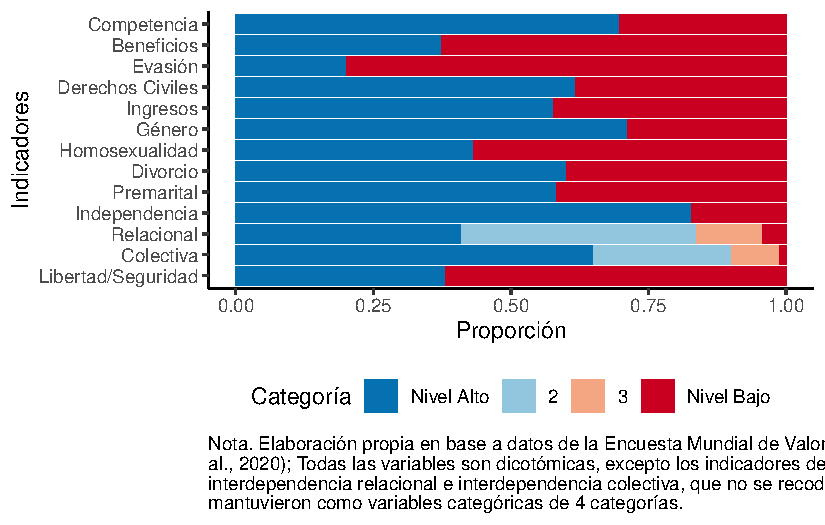
\includegraphics[keepaspectratio]{paper_files/figure-pdf/fig-descriptivos-1.pdf}}

}

\caption{\label{fig-descriptivos}Análisis descriptivo indicadores de
Individualismo}

\end{figure}%

El 83\% declara sentirse a cargo de su propia vida, lo que denota un
alto nivel de autonomía en la población. Asimismo, el 84\% considera que
hacer sentir orgullosos a sus padres es uno de los principales objetivos
en la vida. Además, el 90\% se siente cercano o muy cercano al país. En
conjunto, estos resultados son coherentes con la evidencia previa que
indica que las autoconcepciones independientes e interdependientes no
son excluyentes, sino que coexisten y alcanzan niveles igualmente altos
en Chile (\citeproc{ref-benavides2020}{Benavides y Hur 2020};
\citeproc{ref-kolstad2009}{Kolstad y Horpestad 2009}).

Por último, una proporción importantes de la población (82\%) prioriza
la seguridad (en rojo en la Figura~\ref{fig-descriptivos}) por sobre la
libertad (en azul). Este hallazgo podría representar evidencia a favor
de que la autonomía no es el valor principal en base al cual las
personas no se constituyen como individuos en Chile
(\citeproc{ref-martuccelli2010}{Martuccelli 2010}).

\subsection{Perfiles de
Individualismo}\label{perfiles-de-individualismo}

Se seleccionó un modelo de 4 clases a partir de criterios estadísticos y
teóricos. Como se puede ver en la la Figura~\ref{fig-lca}, las cuatros
clases muestran patrones claramente distintos entre sí, así como
diferencias respecto a la distribución promedio de la muestra.

\begin{figure}[H]

\centering{

\pandocbounded{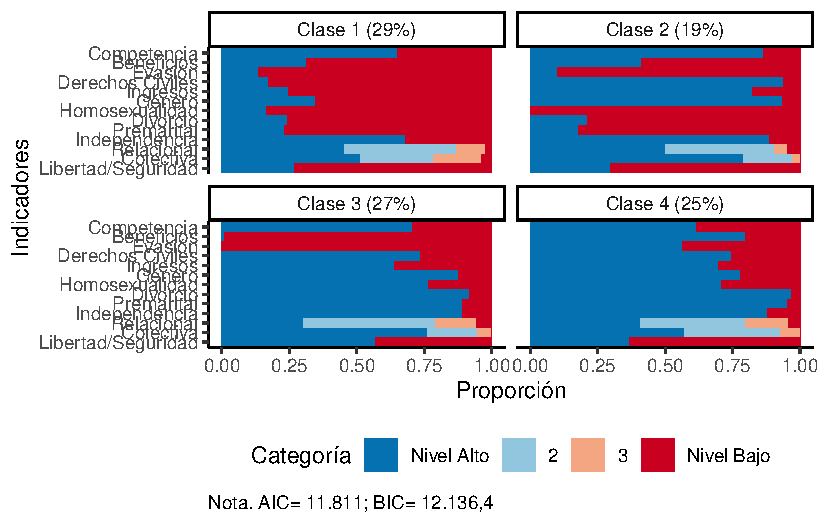
\includegraphics[keepaspectratio]{paper_files/figure-pdf/fig-lca-1.pdf}}

}

\caption{\label{fig-lca}Modelo de clases latentes de individualismo}

\end{figure}%

\subsubsection{Clase 1: Individualistas
Autoritarios}\label{clase-1-individualistas-autoritarios}

La clase 1, que representa el 29\% de la muestra, se caracteriza por
valorar positivamente la competencia, pero a la vez tiende a rechazar la
acción individual en diversas esferas. Por ejemplo, se observa un alto
rechazo a evadir en el transporte público (88\%), una mayor indiferencia
hacia los derechos civiles (83\%) y un rechazo a la homosexualidad
(84\%). Dicho en otras palabras, la acción individual cuenta con baja
legitimidad tanto en la esfera económica, como en la política y en la
expresiva. Para este grupo, la individualidad debe estar subsumida al
respeto irrestricto a las normas socailes establecidas. Asimismo, la
probabilidad de que los miembros de esta clase prefieren la seguridad
por sobre la libertad es la más alta entre las 4 clases, con un 73\%.

Pese a esta desconfianza generalizada hacia la acción individual y la
autonomía, este grupo igualmente muestra un porcentaje relativamente
alto de independencia, con un 68\%. No es, pues, que se niegue la
indivualidad, sino que se concibe que esta debe estar siempre subsumida
al respeto irrestrico a las normas sociales establecidas. Dado que la
conformidad es una característica fuertemente asociada a las
personalidades autoritarias (\citeproc{ref-zakrisson2005}{Zakrisson
2005}), se ha decidido bautizar a este perfil como
\textbf{individualismo autoritario}.

La edad promedio de este grupo es de 46,3 años, ligeramente superior al
promedio de la muestra (44,3 años). Además, este grupo muestra una mayor
religiosidad en términos nominales, con un 67\% de ellos identificandose
como católicos.

\subsubsection{Clase 2: Individualistas
Conservadores}\label{clase-2-individualistas-conservadores}

La clase 2 (19\% de la muestra) se caracteriza por una alta probabilidad
de justificar la competencia y de legitimar la acción individual en la
esfera política, mientras rechaza tanto la acción estratégica como la
individualidad en la esfera expresiva. Esto se ve reflejado en las altas
probabilidades, mayores que las del resto de los grupos, de rechazar la
homosexualidad (100\%), el divorcio (79\%) y el sexo premarital (82\%).

Pese a compartir este último rasgo con el individualismo autoritario,
difieren significativamente en cuanto a la valoración de la acción
individual en la esfera política. Por ejemplo, la probabilidad de
presentar una alta valoración de los derechos civiles alcanza un 93\%
entre la clase 2, la más alta entre las cuatros clases, como se aprecia
en la Figura~\ref{fig-ind-moral}.

\begin{figure}[H]

\centering{

\pandocbounded{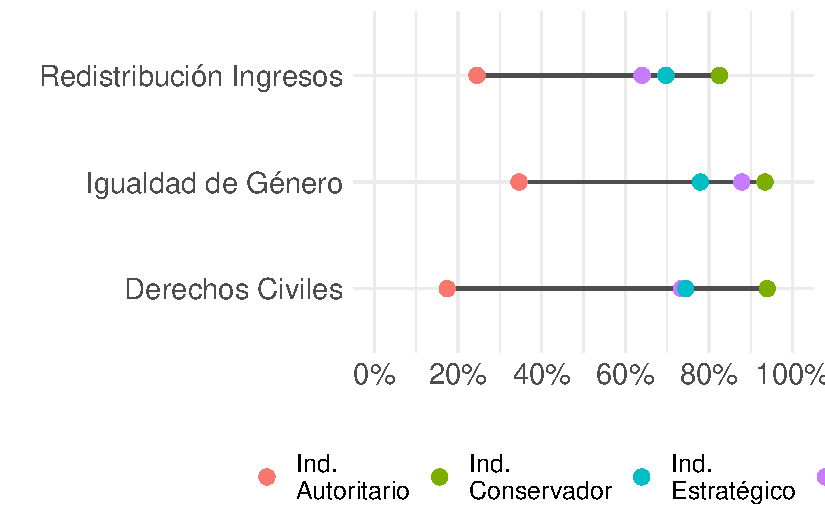
\includegraphics[keepaspectratio]{paper_files/figure-pdf/fig-ind-moral-1.pdf}}

}

\caption{\label{fig-ind-moral}Probabilidad de legitimar acción
individual en la esfera política}

\end{figure}%

Es por la mezcla entre el rechazo a una individualidad expresiva pero la
valoración de la individualidad política es que se ha denominado a este
grupo como \textbf{individualismo conservador}. Los individualistas
conservadores se caracterizan por tener 47,8 años en promedio, se
encuentran políticamente más a la derecha y son mayoritariamente
católicos (63\%).

\subsubsection{Clase 3: Individualistas
Liberales}\label{clase-3-individualistas-liberales}

Esta clase, el 27\% de la muestra, tiene algunos rasgos similares con el
individualismo conservador. Por ejemplo, muestra una alta probabilidad
de legitimar la competencia así como la acción individual en la esfera
política, mientras rechaza las acciones estratégicas.

Sin embargo, se diferencia de la variante anterior en dos aspectos
principales. Por un lado, en la alta legitimidad otorgada a la
individualdad en la esfera expresiva: 76\% justifica la homosexualidad,
91\% el divorcio y 89\% el sexo premarital. Por otro lado, este grupo se
destaca como la única clase donde la probabilidad de elegir la libertad
es mayor que la de preferir la seguridad (57\%).

\begin{figure}[H]

\centering{

\pandocbounded{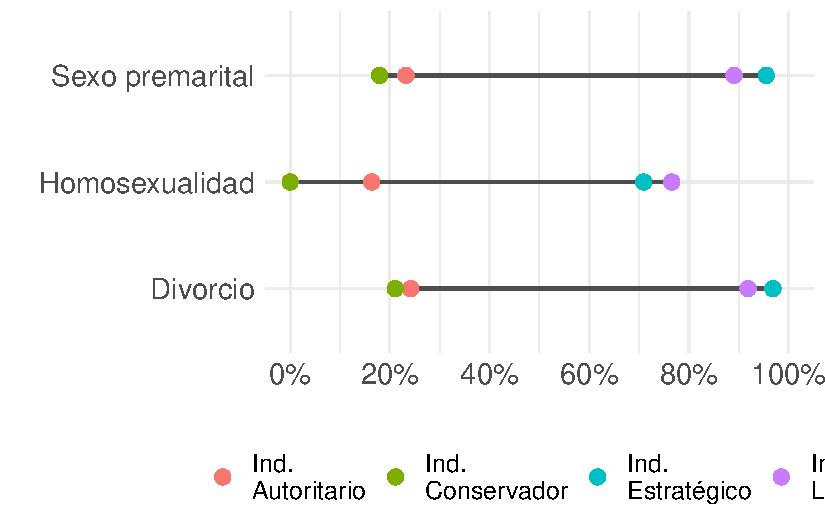
\includegraphics[keepaspectratio]{paper_files/figure-pdf/fig-ind-expresivo-1.pdf}}

}

\caption{\label{fig-ind-expresivo}Probabilidad de legitimar acción
individual en la esfera expresiva}

\end{figure}%

De tal modo, se ha denominado a esta clase como \textbf{individualismo
liberal}, pues, sus valores apuntan al respeto a la libertad y a la
tolerancia de la acción individual en todas las esferas de la vida
social, aunque manteniendo el respeto por algunas normas básicas de
convivencia. Los individualistas liberales tiene una mayor proporción de
personas en la izquierda y centro izquierda del espectro político
(28\%), pero también es el que alberga la mayor cantidad de personas sin
identificación política. Por otro lado, en contraste con las dos clases
anteriores, este grupo es menores religioso, con un 36\% de sus miembros
declarando no tener afiliación religiosa.

\subsubsection{Clase 4: Individualistas
Estratégicos}\label{clase-4-individualistas-estratuxe9gicos}

Finalmente, la clase 4 (25\% de la muestra) se caracteriza por ser el
único perfil en donde se observa una alta probabilidad de legitimar la
acción individual en todas las esferas, incluso si esto implica
transgredir las normas sociales, como se aprecia en la
Figura~\ref{fig-ind-econ}. Por esta razón, se ha decidio denominar a
este perfil como \textbf{individualismo estratégico}.

\begin{figure}[H]

\centering{

\pandocbounded{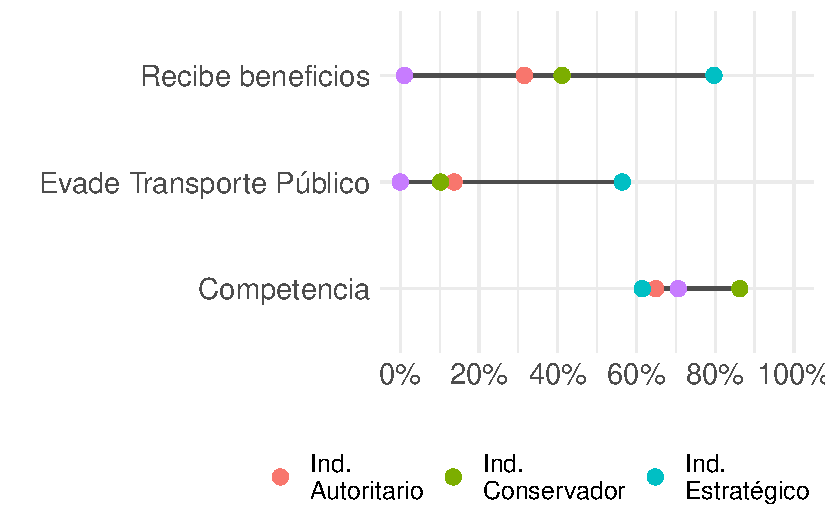
\includegraphics[keepaspectratio]{paper_files/figure-pdf/fig-ind-econ-1.pdf}}

}

\caption{\label{fig-ind-econ}Probabilidad de legitimar acción individual
en la esfera económica}

\end{figure}%

De los cuatro perfiles, este es el único donde se observan diferencias
en la composición de género, mostrando una leve feminización (56\%).
Además, es el grupo más joven, con una edad promedio de 40,3 años.
Comparte con el individualismo liberal una baja identificación
religiosa, ya que el 37\% de sus miembros declara no tener una religión.

\section*{Discusión}\label{discusiuxf3n}
\addcontentsline{toc}{section}{Discusión}

A partir de los datos examinados, se lgró identificar cuatro perfiles
distintos de individaulismo en la sociedad chilena: individualismo
autoritario, individualismo conservador, individualismo liberal e
individualismo estratégico. Cada uno de estos perfiles equivale a
variadas definciiones de la posición del individuo en la sociedad, y son
resultado de combinaciones específicas de legitimdiad de la acción
individual en diferentes esferas, concepciones variadas del individuo y
diferentes valores priorizados. Además, la presencia de dieferencias
edad, orientación política y afiliación religiosa entre estos perfiles
arroja luces sobre cómo los procesos estructruales de individuación
pueden interactuar de manera diferenciada con distintos segmentos de la
población.

La tipología elaborada permite establecer un diálogo con la descripción
del individualismo agéntico y el hiper-actor relacional propuesto por
Araujo y Martuccelli (\citeproc{ref-araujo2020}{Araujo y Martuccelli
2020a}). Este modelo presenta dos características fundamentales: en
primer lugar, la confianza depositada en las habilidades personales para
afrontar la vida social. En segundo lugar, la centralidad de las redes
interpersonales. Estos dos rasgos son observables de manera transversal
en los cuatro perfiles identificados.

En relación con la confianza en el esfuerzo y las habilidades
personales, esto podría observarse en la alta valoración de la
competencia y los elevados niveles de independencia observados de manera
transversal en todos los perfiles, como se observa en
Figura~\ref{fig-concepciones}. En términos generales, los datos sugieren
que la mayoría de los chilenos cree poseer las habilidades necesarias
para asumir el control de sus propias vidas.

\begin{figure}[H]

\centering{

\pandocbounded{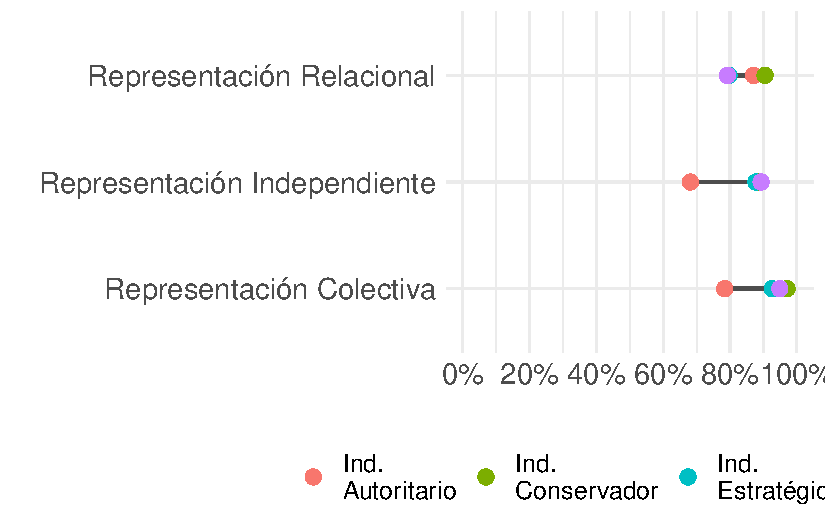
\includegraphics[keepaspectratio]{paper_files/figure-pdf/fig-concepciones-1.pdf}}

}

\caption{\label{fig-concepciones}Representaciones sociales del
individuo}

\end{figure}%

Lo mismo sucede con los altos niveles de interdependencia observados a
través de los cuatro perfiles, poniendo en relieve el carácter
relacional del individualismo chileno. Los individuos en Chile, de tal
modo, no se constituyen de manera atomizada, sino también en relación a
sus familias y a sus identidadades colectivas.

De tal modo, se observa que el carácter relacional del individualismo
chileno parece no entrar en contradicción con las concepciones
independientes, que muestran niveles tan elevados como los de
interdependencia. Esto es consistente tanto con las dos carácteristas
que describen al individualismo agéntico
(\citeproc{ref-araujo2020}{Araujo y Martuccelli 2020a}) como con las
mediciones del \emph{self-construal} en Chile
(\citeproc{ref-benavides2020}{Benavides y Hur 2020};
\citeproc{ref-kolstad2009}{Kolstad y Horpestad 2009}). Además, ofrece
más respaldo a la idea de que ubicar a Chile en un continuo entre el
individualismo y el colectivismo resulta problemático.

En resumen, los datos analizados parecen apuntar a la existncia de un
individualismo agéntico (\citeproc{ref-araujo2020}{Araujo y Martuccelli
2020a}), que representaría una suerte de modelo ideal del individualismo
en Chile. Sin embargo, el aporte de esta investigación radica e que,
mediante el análisis de clases latentes, es posible observar cómo este
modelo diverge dentro de la sociedad chilena. Para algunos, la acción
individual debe estar subordinada al orden normativo, mientras que para
otros es legítimo actuar de manera estratégica incluso si ello
transgrede normas sociales. Mientras que para unos la individualidad
tiene cabida en todas las esferas, para otros su legitimidad no alcanza
para la esfera afectiva. De tal modo, este enfoque permite observar los
matics y las divergencias de los procesos de individualización en Chile.

\section{Conclusiones}\label{conclusiones}

Es importante reflexionar sobre las oportunidades que brinda el análisis
de clases latentes en la investigación sobre los procesos de
individuación en Chile. Dada la dificultad para traducir su marco
teórico en una propuesta metodológica mediante las técnicas
cuantitativas más comunes, la sociología del individuo se ha
desarrollado principalmente desde una perspectiva cualitativa,
resultando en descripciones profundas y estimulantes sobre el indiudo en
la sociedad chilena. Pese a ello, el enfoque metodológico adoptado en
esta investigación, caracterizado por la aproximación orientada a la
personas del modeeo de clases latentes, permitió identificar algunos de
los rasgos del individualismo agéntico descritos por Araujo y
Martuccelli (\citeproc{ref-araujo2014}{2014}), al tiempo que ofrece una
visión más matizada de cómo los procesos de individuación divergen en la
sociedad chilena.

Por supuesto, enfoques cualitativos y cuantitativos no deben ser vistos
como competitivos, sino como complementarios en el desarrollo de una
sociología del individuo. La propia tipología aquí delineada se vería
fuertemente enriquecida si se incluyeran datos cualitativos que
permitieran una comprensión más profunda de las distintas variables de
individualismo.

Ahora bien, es necesario reconocer las limitaciones que enfrentó esta
investigación, principalmente derivadas de los indicadores
seleccionados. Aunque los resultados obtenidos son prometedores, es
crucial continuar avanzado en la construcción y validación de
indicadores que permitan traducir el modelo teórico aquí propuesto en un
modelo de medición capaz de abordar el fenómeno del individualismo en
Chile.

Especialmente, se debe tener en cuenta que la recodificación de
variables continuas como dicotómicas es una solución correcta, pero que
no deja de ser problemática, pues resulta en pérdida de parte de la
varianza de los ítems (\citeproc{ref-fernandes2019}{Fernandes et~al.
2019}). Futuras investigaciones deberían considerar elaborar indicadores
directamente como variables categóricas que no necesiten recodificación
para ser incluidas en el modelo de clases latentes. De esta manera, se
obtentendría claridad en los resultados sin sacrificar información ni
poder estadístico.

Por otro lado, se debe considerar que la muestra utilizada es del 2018,
por lo que no alcanza a aprehender las consecuencias de procesos y
eventos sociles de agran relevancia acontecidos en el último lustro,
incluyendo el Estallido Social, la Pandemia de COVID-19 y los procesos
constituyentes. Una nueva ola de la Encuesta Mundial de Valores se
encuentra en desarrolo, lo que dará una oportunidad para probar este
modeeo con datos actualizados. A su vez, dado que Chile ha participado
en 6 olas de la Encuesta Mundial de Valores desde 1990, se debería
considerar un estudio comparativos a partir de datos de ediciones
anteriores.

Pese a estas limitaciones, el modelo propuesto logra identificar
variantes de individualismo, ilustrando tanto la dificultad para ubicar
a la sociedad chilena en un espectro individualismo-colectivismo, al
mismo tiempo que matiza las descripciones unívocas del individualismo
chileno. Esto abre la posibilidad para profundizar en este modelo en el
futuro, particularmente en su interacción con otros fenómenos sociales.

Por dar solo un ejemplo, en el más reciente Informe sobre el Desarrollo
Humano en Chile (\citeproc{ref-pnud2024}{PNUD 2024}) se identifica a la
individualismo asocial coo una de las lógicas inhibidoras para conducir
el cambio social en el país. ¿Es esa individuación asocial homogénea
dentro de la sociedad chilena? ¿Se asocian distintas formas de
individuación e individualismo con diferentes maneras de relacionarse
con el espacion público? ¿Qué factores explican essas divergencias? El
modelo aquí propueso podría dar algunas luces para responder estas
preguntas, permitiendo entender mejor como el individualismo se
relaciona con la esfera pública, la democracia y la participación
política.

\phantomsection\label{refs}
\begin{CSLReferences}{1}{0}
\bibitem[\citeproctext]{ref-araujo2012}
Araujo, Kathya, y Danilo Martuccelli. 2012. \emph{Desaf{í}os {Comunes}.
{Retrato} de La Sociedad Chilena y Sus Individuos}. LOM.

\bibitem[\citeproctext]{ref-araujo2014}
---------. 2014. {«Beyond Institutional Individualism: {Agentic}
Individualism and the Individuation Process in {Chilean} Society»}.
\emph{Current Sociology} 62 (1): 24-40.
\url{https://doi.org/10.1177/0011392113512496}.

\bibitem[\citeproctext]{ref-araujo2020}
---------. 2020a. {«Leer Los Movimientos Sociales Desde El
Individualismo: {Reflexiones} a Partir de {Latinoam{é}rica}»}.
\emph{Educa{ç}{ã}o \& Sociedade} 41: e228265.
\url{https://doi.org/10.1590/es.228265}.

\bibitem[\citeproctext]{ref-araujo2020a}
---------. 2020b. {«Problematizaciones Del Individualismo En {Am{é}rica
Latina}»}. \emph{Perfiles Latinoamericanos} 28 (55).
\url{https://doi.org/10.18504/pl2855-001-2020}.

\bibitem[\citeproctext]{ref-baeza2022}
Baeza, Jorge, y Patricia Imbarack. 2022. {«{Movilidad religiosa en
j{ó}venes universitarios de Chile: desafiliaciones y reafiliaciones en
la iglesia cat{ó}lica}»}. \emph{Religi{ã}o \& Sociedade} 42 (3): 60-83.
\url{https://doi.org/10.1590/0100-85872022v42n3cap03}.

\bibitem[\citeproctext]{ref-benavides2020}
Benavides, Paloma, y Taekyun Hur. 2020. {«Self-{Construal Differences}
in {Chile} and {South Korea}: {A Brief Report}»}. \emph{Psychological
Reports} 123 (6): 2410-17.
\url{https://doi.org/10.1177/0033294119868786}.

\bibitem[\citeproctext]{ref-bergman2015}
Bergman, Lars R., y Lars-Gunnar Lundh. 2015. {«Introduction: {The}
Person-Oriented Approach: {Roots} and Roads to the Future»}.
\emph{Journal for Person-Oriented Research} 1 (1-2): 1-6.
\url{https://doi.org/10.17505/jpor.2015.01}.

\bibitem[\citeproctext]{ref-brewer2007}
Brewer, Marilynn B., y Ya-Ru Chen. 2007. {«Where ({Who}) {Are
Collectives} in {Collectivism}? {Toward Conceptual Clarification} of
{Individualism} and {Collectivism}.»} \emph{Psychological Review} 114
(1): 133-51. \url{https://doi.org/10.1037/0033-295X.114.1.133}.

\bibitem[\citeproctext]{ref-canalesceron2021}
Canales Cerón, Manuel, Víctor Sebastián Orellana Calderón, y Fabián
Guajardo Mañán. 2021. {«Sujeto y Cotidiano En La Era Neoliberal: El Caso
de La Educaci{ó}n Chilena»}. \emph{Revista Mexicana de Ciencias
Pol{í}ticas y Sociales} 67 (244): 285-307.
\url{https://doi.org/10.22201/fcpys.2448492xe.2022.244.70386}.

\bibitem[\citeproctext]{ref-castillo_cohesion_2022}
Castillo, Juan Carlos, Vicente Espinoza, y Emmanuelle Barozet. 2022.
{«{Cohesi{ó}n social en Chile en tiempos de cambio: indicadores,
perfiles y factores asociados}»}.

\bibitem[\citeproctext]{ref-castillo_socialization_2024}
Castillo, Juan Carlos, Mauricio Salgado, Kevin Carrasco, y Andreas
Laffert. 2024. {«The {Socialization} of {Meritocracy} and {Market
Justice Preferences} at {School}»}. \emph{Societies} 14 (11): 214.
\url{https://doi.org/10.3390/soc14110214}.

\bibitem[\citeproctext]{ref-collins2010}
Collins, Linda, y Stephanie Lanza. 2010. \emph{Latent Class and Latent
Tansition Analysis.} Wiley.

\bibitem[\citeproctext]{ref-cortesparedes_autonomia_2022}
Cortés Paredes, Gabriel. 2022. {«Autonom{í}a En El Horizonte: Un
An{á}lisis Narrativo de Los Procesos de Deconversi{ó}n En {Temuco},
{Chile}»}. \emph{Revista Temas Sociol{ó}gicos}, n.º 30: 75-105.
\url{https://doi.org/10.29344/07196458.30.3122}.

\bibitem[\citeproctext]{ref-cortois2018}
Cortois, Liza, y Rudi Laermans. 2018. {«Rethinking Individualization:
{The} Basic Script and the Three Variants of Institutionalized
Individualism»}. \emph{European Journal of Social Theory} 21 (1): 60-78.
\url{https://doi.org/10.1177/1368431017698474}.

\bibitem[\citeproctext]{ref-cross2011}
Cross, Susan E., Erin E. Hardin, y Berna Gercek-Swing. 2011. {«The
{\emph{What}}{\emph{,} }{\emph{How}}{\emph{,} }{\emph{Why}}{\emph{, and}
}{\emph{Where}} of {Self-Construal}»}. \emph{Personality and Social
Psychology Review} 15 (2): 142-79.
\url{https://doi.org/10.1177/1088868310373752}.

\bibitem[\citeproctext]{ref-fernandes2019}
Fernandes, Antônio, Caio Malaquias, Dalson Figueiredo, Enivaldo Da
Rocha, y Rodrigo Lins. 2019. {«Why {Quantitative Variables Should Not Be
Recoded} as {Categorical}»}. \emph{Journal of Applied Mathematics and
Physics} 07 (07): 1519-30.
\url{https://doi.org/10.4236/jamp.2019.77103}.

\bibitem[\citeproctext]{ref-gayo_individuo_2017}
Gayo, Modesto. 2017. {«{El individuo frente a la sociedad o el western
sociol{ó}gico}»}. \emph{Estudios P{ú}blicos}, n.º 147: 263-79.

\bibitem[\citeproctext]{ref-kolstad2009}
Kolstad, Arnulf, y Silje Horpestad. 2009. {«Self-{Construal} in {Chile}
and {Norway}: {Implications} for {Cultural Differences} in
{Individualism} and {Collectivism}»}. \emph{Journal of Cross-Cultural
Psychology} 40 (2): 275-81.
\url{https://doi.org/10.1177/0022022108328917}.

\bibitem[\citeproctext]{ref-leonquillas2022}
León Quillas, César Ignacio, Héctor Fernando Rueda Rodríguez, y
Alejandra Hernández Rodríguez. 2022. {«Instituciones Informales,
Emprendimiento y Progreso Social: Un Estudio Comparativo y
Correlacional»}. \emph{Revista Guillermo de Ockham} 21 (1): 113-29.
\url{https://doi.org/10.21500/22563202.5577}.

\bibitem[\citeproctext]{ref-linzer2011}
Linzer, Drew A., y Jeffrey B. Lewis. 2011. {«{poLCA}: {An R Package} for
{Polytomous Variable Latent Class Analysis}»}. \emph{Journal of
Statistical Software} 42 (junio): 1-29.
\url{https://doi.org/10.18637/jss.v042.i10}.

\bibitem[\citeproctext]{ref-martuccelli2010}
Martuccelli, Danilo. 2010. \emph{{{\textquestiondown}Existen individuos
en el sur?}} Santiago de Chile: LOM.

\bibitem[\citeproctext]{ref-martuccelli2018}
---------. 2018. {«Variantes Del Individualismo»}. \emph{Estudios
Sociol{ó}gicos de El Colegio de M{é}xico} 37 (109): 7-37.
\url{https://doi.org/10.24201/es.2019v37n109.1732}.

\bibitem[\citeproctext]{ref-mideso_informe_2020}
Ministerio de Desarrollo Social y Familia. 2020. {«Informe {Final
Consejo Asesor} Para La {Cohesi{ó}n Social}. {Diagn{ó}stico} Para Una
Aproximaci{ó}n a La Cohesi{ó}n Social En {Chile} y Recomendaciones Para
Fortalecer El Aporte de La Pol{í}tica Social»}.

\bibitem[\citeproctext]{ref-moemeka1998}
Moemeka, Andrew A. 1998. {«Communalism as a {Fundamental Dimension} of
{Culture}»}. \emph{Journal of Communication} 48 (4): 118-41.
\url{https://doi.org/10.1111/j.1460-2466.1998.tb02773.x}.

\bibitem[\citeproctext]{ref-murray2022}
Murray, Marjorie, y Constanza Tizzoni. 2022. {«Raising Children in
Hostile Worlds in {Santiago} de {Chile}: {Optimism} and
{``Hyper-Agentic''} Mothers»}. \emph{The Sociological Review} 70 (1):
92-107. \url{https://doi.org/10.1177/00380261211056169}.

\bibitem[\citeproctext]{ref-oyserman2002}
Oyserman, Daphna, Heather M. Coon, y Markus Kemmelmeier. 2002.
{«Rethinking Individualism and Collectivism: {Evaluation} of Theoretical
Assumptions and Meta-Analyses.»} \emph{Psychological Bulletin} 128 (1):
3-72. \url{https://doi.org/10.1037/0033-2909.128.1.3}.

\bibitem[\citeproctext]{ref-pinheiro2023}
Pinheiro, Leandro R., Pablo Francisco Di Leo, y Francisco Ramírez
Varela. 2023. {«{Itinerarios juveniles, individuaci{ó}n y
reflexividades: aproximaciones a la participaci{ó}n social en barrios
metropolitanos populares}»}. \emph{Educa{ç}{ã}o e Pesquisa} 49.
\url{https://doi.org/10.1590/s1678-4634202349270569es}.

\bibitem[\citeproctext]{ref-pnud2024}
PNUD. 2024. {«Informe Sobre {Desarrollo Humano} En {Chile} 2024.
{\textquestiondown}{Por} Qu{é} Nos Cuesta Cambiar?: Conducir Los Cambios
Para Un {Desarrollo Humano Sostenible}»}. Santiago de Chile.

\bibitem[\citeproctext]{ref-robles2001}
Robles, Fernando. 2001. \emph{El Desaliento Inesperado de La Modernidad:
{Molestias}, Irritaciones y Frutos Amargos de La Sociedad Del Riesgo}.
Sociedad de Hoy.

\bibitem[\citeproctext]{ref-rojas2008}
Rojas-Méndez, José I., Vilma Coutiño-Hill, Rabi S. Bhagat, y Karen South
Moustafa. 2008. {«{Evaluaci{ó}n del individualismo y colectivismo
horizontal y vertical en la sociedad Chilena.}»} \emph{Multidisciplinary
Business Review} 1 (1): 36-48.

\bibitem[\citeproctext]{ref-salazar-xirinachs_repensar_2023}
Salazar-Xirinachs, José Manuel. 2023. {«{Repensar, reimaginar,
transformar: los {``qu{é}''} y los {``c{ó}mo''} para avanzar hacia un
modelo de desarrollo m{á}s productivo, inclusivo y sostenible}»}.
\emph{Revista de la CEPAL} 2023 (141): 11-43.
\url{https://doi.org/10.18356/16820908-2023-141-2}.

\bibitem[\citeproctext]{ref-silvapalacios2015}
Silva Palacios, Vicente. 2015. {«Narrativas de {Individualizaci{ó}n} En
{Chile}»}. Tesis de \{\{Pregrado\}\}, Universidad de Chile.

\bibitem[\citeproctext]{ref-solsona-cisternas2023}
Solsona-Cisternas, Diego Alfredo. 2023. {«Individuation Processes in
Disabled People. {An} Approach Through Mobilities in Rural Areas of
Southern {Chile}»}. \emph{Disability \& Society}, 1-23.
\url{https://doi.org/10.1080/09687599.2023.2263632}.

\bibitem[\citeproctext]{ref-soto2021}
Soto, Álvaro, Antonio Stecher, y Pamela Frías. 2021.
{«{\textquestiondown}{Nuevas} Orientaciones Subjetivas En El Trabajo?
{Los} J{ó}venes de La Industria Del Retail En {Chile}»}. \emph{Athenea
Digital. Revista de pensamiento e investigaci{ó}n social} 21 (1).
\url{https://doi.org/10.5565/rev/athenea.2772}.

\bibitem[\citeproctext]{ref-trebilcock2019}
Trebilcock, Maria Paz, y Alejandra Luneke. 2019. {«Crime {Prevention}
and the {Coproduction} of {Security}: {Outcomes} of {Citizen
Participation} at the {Neighborhood Level} in {Neoliberal Chile}»}.
\emph{Latin American Perspectives} 46 (6): 56-72.
\url{https://doi.org/10.1177/0094582x18803681}.

\bibitem[\citeproctext]{ref-voronov2002}
Voronov, Maxim, y Jefferson A. Singer. 2002. {«The {Myth} of
{Individualism-Collectivism}: {A Critical Review}»}. \emph{The Journal
of Social Psychology} 142 (4): 461-80.
\url{https://doi.org/10.1080/00224540209603912}.

\bibitem[\citeproctext]{ref-wang2010}
Wang, Georgette, y Zhong-Bo Liu. 2010. {«What Collective? {Collectivism}
and Relationalism from a {Chinese} Perspective»}. \emph{Chinese Journal
of Communication} 3 (1): 42-63.
\url{https://doi.org/10.1080/17544750903528799}.

\bibitem[\citeproctext]{ref-yoon2010}
Yoon, Kwang-Il. 2010. {«Political {Culture} of {Individualism} and
{Collectivism}»}. A \{\{Dissertation\}\} for the \{\{Degree\}\} of
\{\{Doctor\}\} of \{\{Philosophy\}\} (\{\{Political Science\}\}),
Universidad de Michigan.

\bibitem[\citeproctext]{ref-yopo2013}
Yopo, Martina. 2013. {«{Individualizaci{ó}n en Chile. Individuo y
sociedad en las transformaciones culturales recientes}»}.
\emph{Psicoperspectivas. Individuo y Sociedad} 12 (2): 4-15.
\url{https://doi.org/10.5027/psicoperspectivas-Vol12-Issue2-fulltext-254}.

\bibitem[\citeproctext]{ref-zakrisson2005}
Zakrisson, Ingrid. 2005. {«Construction of a Short Version of the
{Right-Wing Authoritarianism} ({RWA}) {Scale}»}. \emph{Personality and
Individual Differences} 39 (octubre): 863-72.
\url{https://doi.org/10.1016/j.paid.2005.02.026}.

\bibitem[\citeproctext]{ref-zhai2022}
Zhai, Yida. 2022. {«Values {Change} and {Support} for {Democracy} in
{East Asia}»}. \emph{Social Indicators Research} 160 (1): 179-98.
\url{https://doi.org/10.1007/s11205-021-02807-3}.

\end{CSLReferences}




\end{document}
